% !TeX root = ../cyh.tex

\chapter{补充内容}

\section{插图}

\begin{figure}[H]
    \centering
    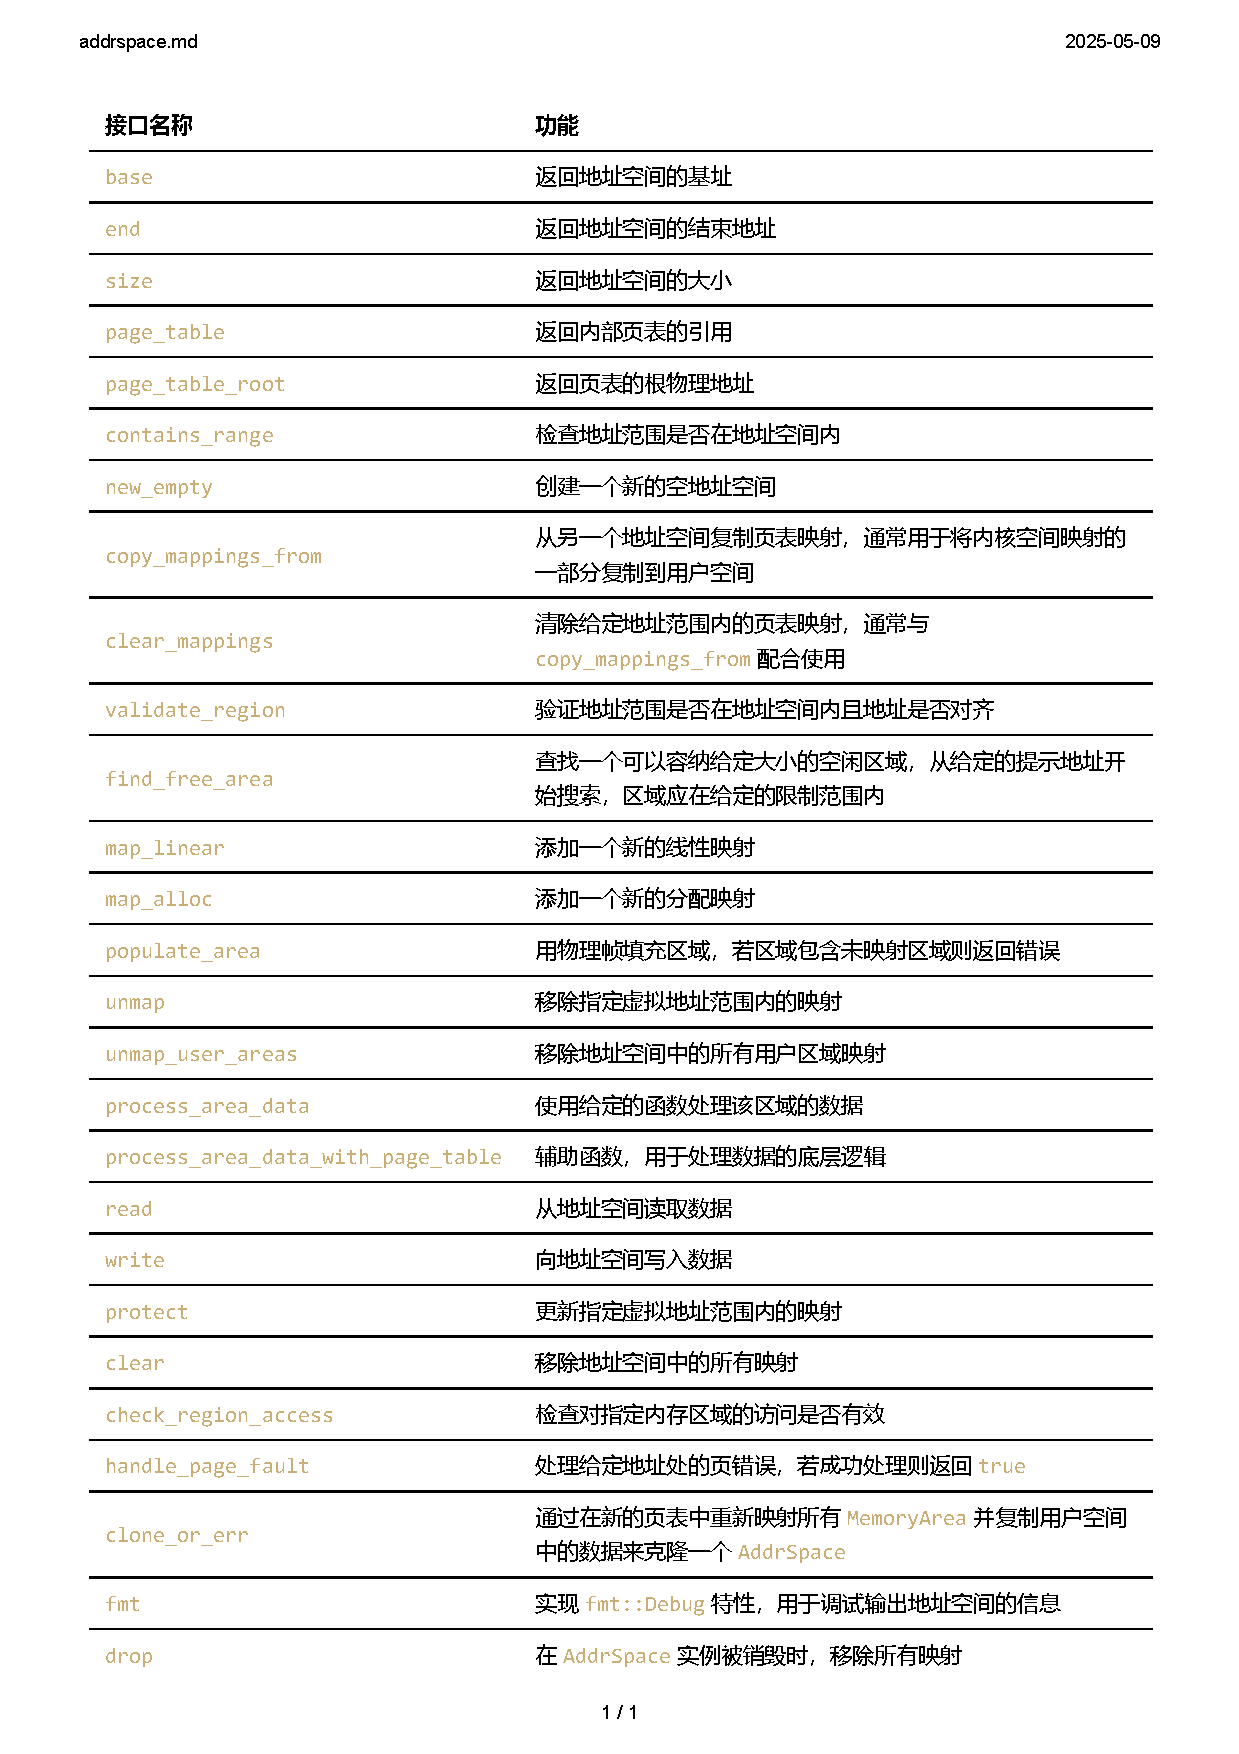
\includegraphics[width=0.9\linewidth]{addrspace.pdf}
    \caption{AddrSpace 结构体接口}
    \label{fig:AddrSpace}
\end{figure}

\begin{figure}
    \centering
    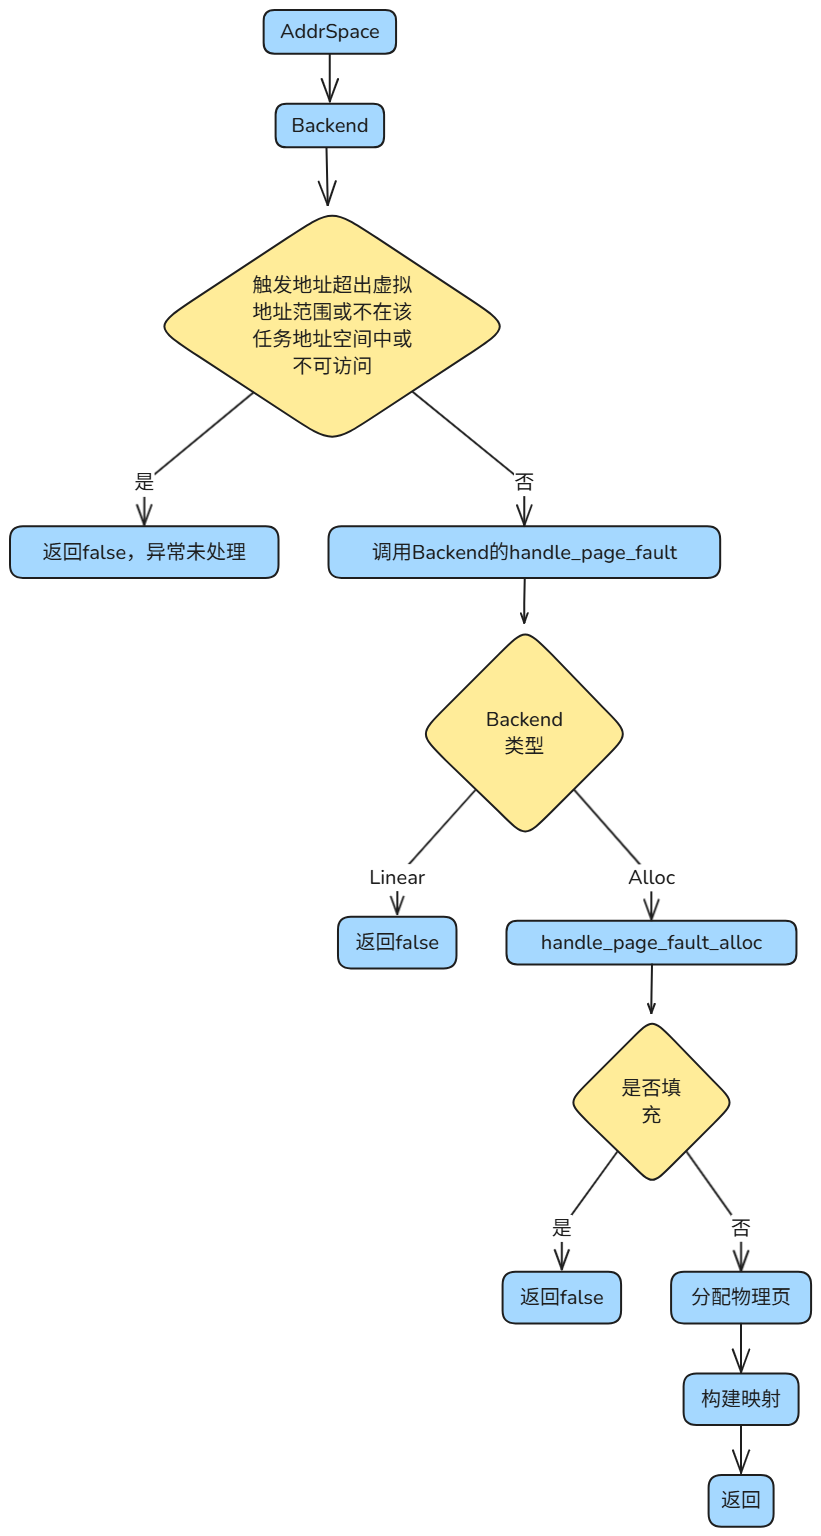
\includegraphics[width=0.7\linewidth,height = 17cm, keepaspectratio]{pagefault-arceos.png}
    \caption{handle\_page\_fault 函数流程图}
    \label{fig:handle-page-fault-arceos}
\end{figure}


\begin{figure}
\centering %图片全局居中
%并排几个图,就要写几个minipage
\begin{minipage}[b]{0.3\textwidth} %所有minipage宽度之和要小于1,否则会自动变成竖排
\centering %图片局部居中
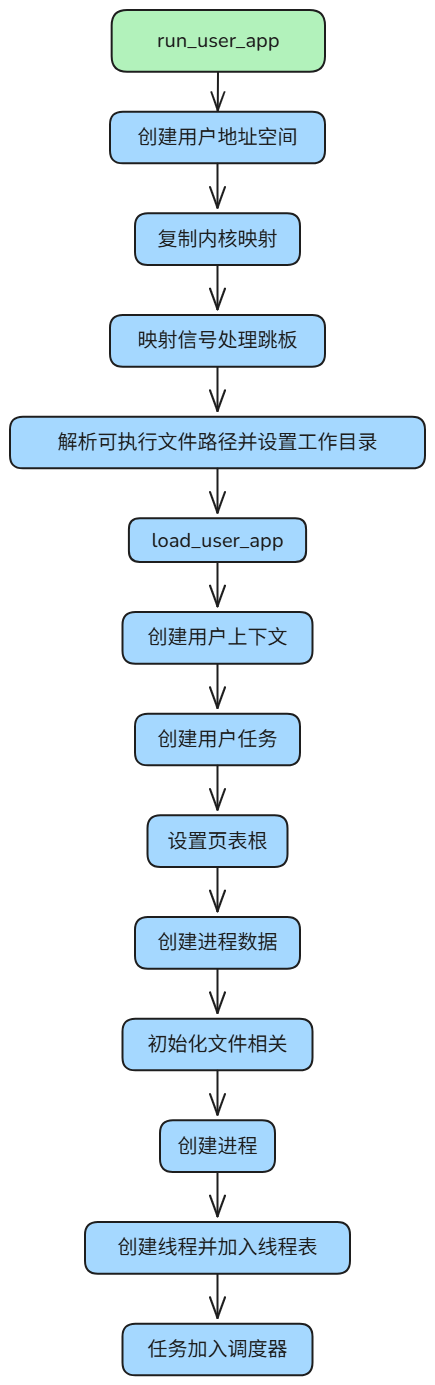
\includegraphics[width=1\textwidth]{run-user-app.png} %此时的图片宽度比例是相对于这个minipage的,不是全局
\caption{run\_user\_app 函数流程图}
\label{fig:run-user-app}
\end{minipage}
\begin{minipage}[b]{0.65\textwidth} %所有minipage宽度之和要小于1,否则会自动变成竖排
\centering %图片局部居中
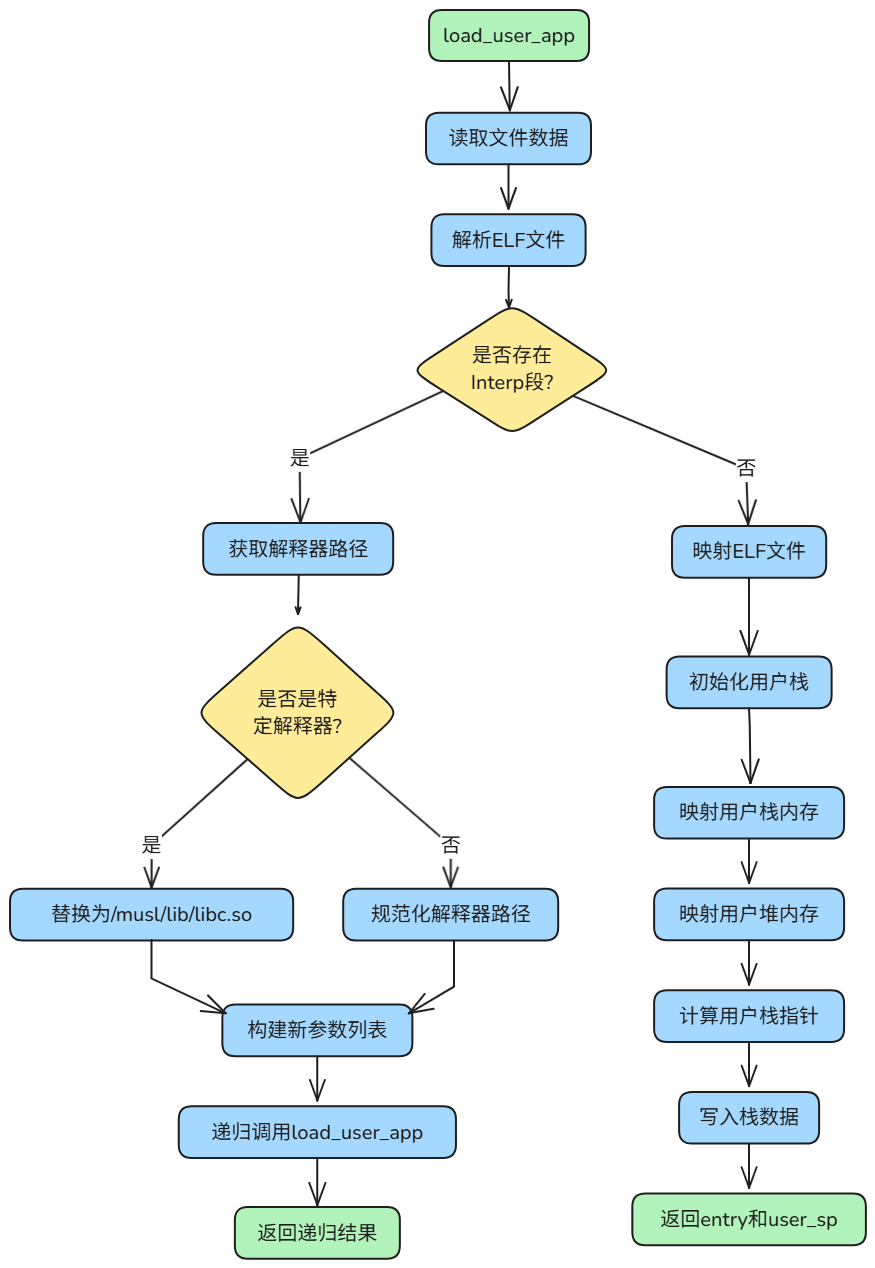
\includegraphics[width=1\textwidth]{load-user-app.png}%此时的图片宽度比例是相对于这个minipage的,不是全局
\caption{load\_user\_app 函数流程图}
\label{fig:load-user-app}
\end{minipage}
\end{figure}